\section{Motivation}
\label{sec:motivation}

As motivation, we present the use case of a simplified todo-list application, created to showcase the functionality and features of \dsl{}.

\subsection{Running Example}

The application has two screens: a main screen and a menu screen. The main screen contains a navigation bar and three todo items. An overview of the application is given in Figure~\ref{fig:appOverview}.

\begin{figure}[!htbp]
\centering
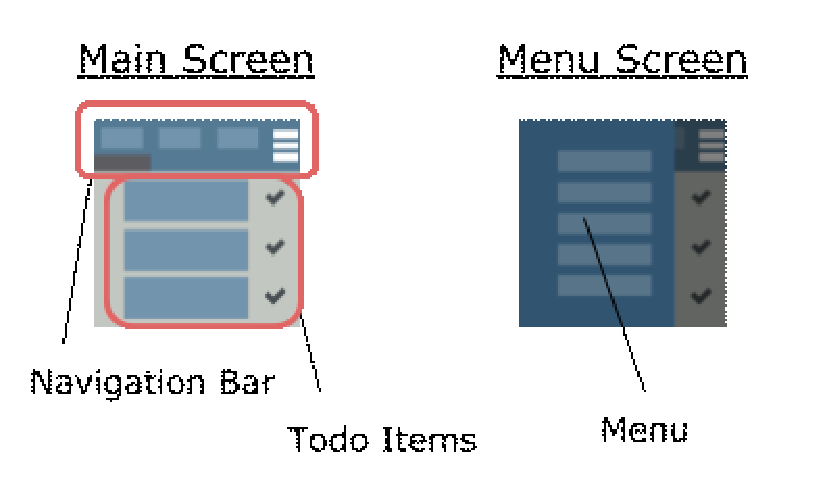
\includegraphics[width=\figscale\textwidth]{pictures/app_overview}
\caption{Overview of the todo-list application.}
\label{fig:appOverview}
\end{figure}

In this application, various user actions are accompanied with an animation:
\begin{itemize}
\item Each todo item can be marked as \emph{done} or \emph{not done} by clicking on it. The checkmark icon changes shape and color to indicate the change in status. These are the \hs{markAsDone}/\hs{markAsNotDone} animations, of which \hs{markAsDone} is shown in Figure~\ref{fig:completeIconCheck}.
\item Todo items can be filtered by their status by using the navigation bar buttons. The first button shows all items, the second shows all complete items, and the third shows all incomplete items. Both the navigation bar underline and the todo items itself change shape to indicate the change in selection. These are the \hs{showAll}/\hs{onlyDone}/\hs{onlyNotDone} animations, of which \hs{onlyDone} is shown in Figure~\ref{fig:onlyDoneFig}.
\item The menu screen shows/hides itself after clicking the hamburger icon. The menu expands inward from the left, to indicate the change in application state. These are the \hs{menuIntro}/\hs{menuOutro} animations, of which \hs{menuIntro} is shown in Figure~\ref{fig:menuIntroFig}.
\end{itemize}

\begin{figure}[!htbp]
\centering

\begin{subfigure}[h]{\textwidth}
\centering
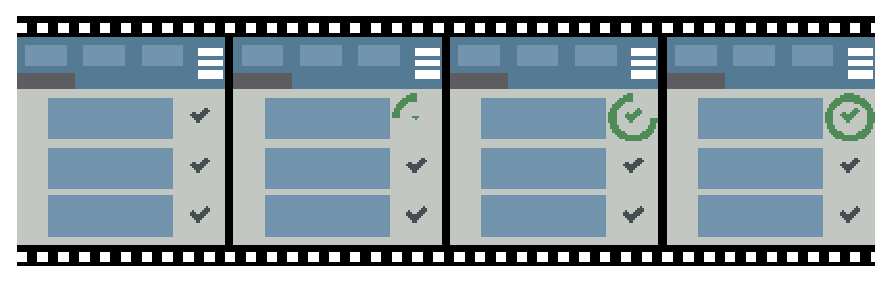
\includegraphics[width=\figscale\textwidth]{pictures/completeIconCheckFig}
\caption{The \hs{markAsDone} animation, the checkmark changes shape and color.}
\label{fig:completeIconCheck}
\end{subfigure}

\begin{subfigure}[h]{\textwidth}
\centering
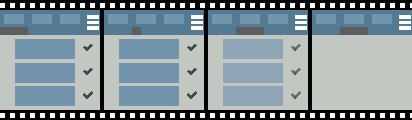
\includegraphics[width=\figscale\textwidth]{pictures/onlyDoneFig}
\caption{The \hs{onlyDone} animation, each of the not done todo items fades out and the navbar underline changes.}
\label{fig:onlyDoneFig}
\end{subfigure}

\begin{subfigure}[h]{\textwidth}
\centering
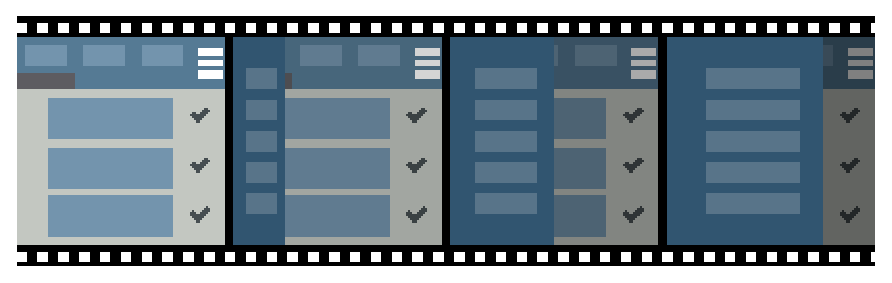
\includegraphics[width=\figscale\textwidth]{pictures/menuIntroFig}
\caption{The \hs{menuIntro} animation, the menu appears while the background fades out.}
\label{fig:menuIntroFig}
\end{subfigure}

\caption{Micro-Animations in the todo application.}
\label{fig:animExamples}
\end{figure}

\subsection{Composing Animations}

The philosophy of \dsl{} is to express animations by combining smaller animations into larger ones. To express an animation, we need to come up with a suitable decomposition. For example, the \hs{menuIntro} animation is composed by combining the two basic animations \hs{menuSlideIn} and \hs{appFadeOut} in parallel. These animations respectively introduce the menu screen and fade out the application in the background.

In the next sections we explain how to construct these basic and composed animations.

\subsection{Basic Animations}

A basic animation changes the value of an element in the UI over a period of time. To specify a basic animation we need three elements: a lens specifying which property in our UI should change, the target value for this property and, lastly, the duration specifying how many seconds the animation should last. Since this operation creates an animation which moves a property \emph{to} a target linearly, it is called \hs{linearTo}.

\paragraph{Note on Lenses} We utilize the lens notation \texttt{x . y . z} to target the property \texttt{z} inside a nested structure \hs{{ x: { y: { z: Property } } }}. This type of lenses were introduced by Twan van Laarhoven \cite{vlLenses}, and newer versions of this idea have been packaged into various Haskell libraries, such as \texttt{lens}\footnote{\url{https://hackage.haskell.org/package/lens}}.

To implement the navigation bar underline animation, we need two basic components for the underline on each button. We reduce the underline width of the first button for 0.25 seconds, and increase the underline width of the second button for 0.25 seconds. These animations are expressed in respectively \hs{line1Outro} and \hs{line2Intro} below, and shown visually in Figure~\ref{fig:basic}.

\begin{spec}
line1Outro = linearTo (navbar . underline1 . width) (For 0.25) (To 0)

line2Intro = linearTo (navbar . underline2 . width) (For 0.25) (To 28)
\end{spec}

We also define the \hs{menuSlideIn} and \hs{appFadeOut} animations below, since we will use these in the next sections. For the former, we increase the width of the menu over a duration of 0.5 seconds, and for the latter we increase the alpha value of the obscuring box over a duration of 0.5 seconds. These animations are shown visually in Figure~\ref{fig:basic}.

\begin{spec}
menuSlideIn = linearTo (menu . width) (For 0.5) (To 75)

appFadeOut = linearTo (obscuringBox . alpha) (For 0.5) (To 0.65)
\end{spec}

\begin{figure}[!htbp]
\centering

\begin{subfigure}[h]{\textwidth}
\centering
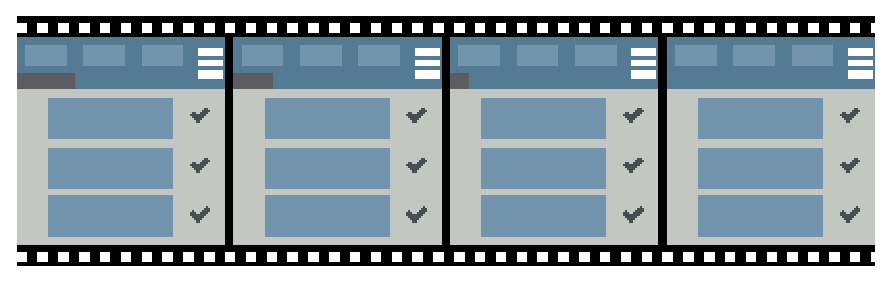
\includegraphics[width=\figscale\textwidth]{pictures/line1OutroFig}
\caption{The \hs{line1Outro} animation.}
\label{fig:basic1_1}
\end{subfigure}

\begin{subfigure}[h]{\textwidth}
\centering
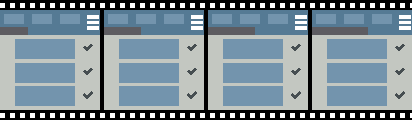
\includegraphics[width=\figscale\textwidth]{pictures/line2IntroFig}
\caption{The \hs{line2Intro} animation.}
\label{fig:basic1_2}
\end{subfigure}

\begin{subfigure}[h]{\textwidth}
\centering
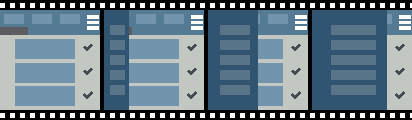
\includegraphics[width=\figscale\textwidth]{pictures/menuSlideInFig}
\caption{The \hs{menuSlideIn} animation.}
\label{fig:basic2_1}
\end{subfigure}

\begin{subfigure}[h]{\textwidth}
\centering
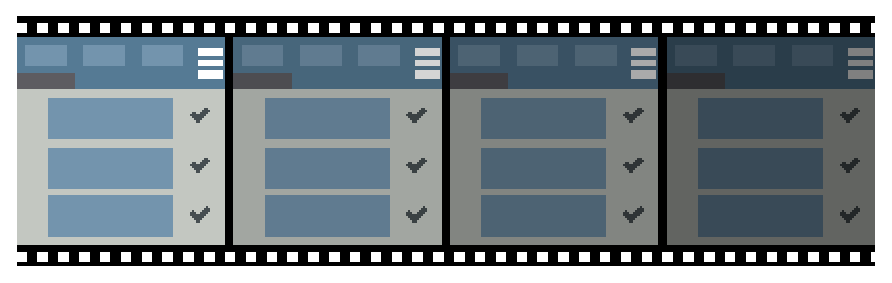
\includegraphics[width=\figscale\textwidth]{pictures/appFadeOutFig}
\caption{The \hs{appFadeOut} animation.}
\label{fig:basic2_2}
\end{subfigure}

\caption{All of the defined basic animations.}
\label{fig:basic}
\end{figure}

\subsection{Composed Animations}

A composed animation combines several other animations into one new animation. We can do this either in \emph{sequence} or in \emph{parallel}.

To obtain the \hs{selectBtn2} animation, we combine the \hs{line1Outro} and \hs{line2Intro} animations with the \hs{sequential} combinator. This constructs a new animation which first plays the \hs{line1Outro} animation, and once it is finished plays the \hs{line2Intro} animation.

\begin{spec}
selectBtn2Anim = line1Outro `sequential` line2Intro
\end{spec}

To obtain the \hs{menuIntro} animation, we combine the \hs{menuSlideIn} and \hs{appFadeOut} animations with the \hs{parallel} combinator. This constructs a new animation wich plays both the \hs{menuSlideIn} and \hs{appFadeOut} animations at the same time.

\begin{spec}
menuIntro = menuSlideIn `parallel` appFadeOut
\end{spec}

Both of these animations are shown visually in Figure~\ref{fig:composed}.

\begin{figure}[!htbp]
\centering

\begin{subfigure}[h]{\textwidth}
\centering
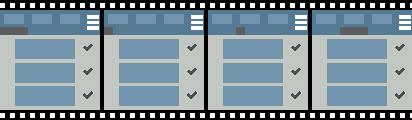
\includegraphics[width=\figscale\textwidth]{pictures/selectBtn2AnimFig}
\caption{The \hs{selectBtn2} animation.}
\label{fig:composed1}
\end{subfigure}

\begin{subfigure}[h]{\textwidth}
\centering
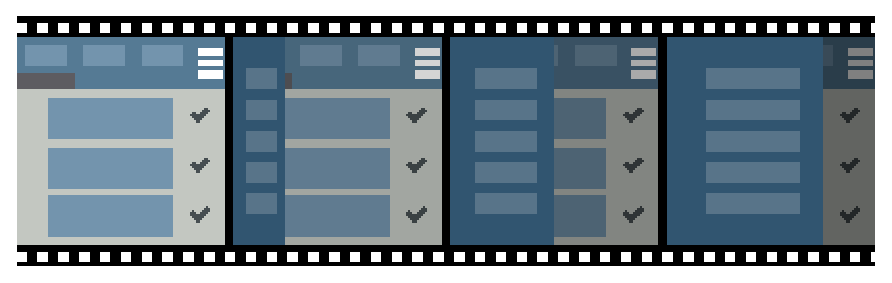
\includegraphics[width=\figscale\textwidth]{pictures/menuIntroFig}
\caption{The \hs{menuIntro} animation.}
\label{fig:composed2}
\end{subfigure}

\caption{All of the defined composed animations.}
\label{fig:composed}
\end{figure}
